\section{采样理论}\label{sec:采样理论}
数字图像表示为一组像素值,通常对齐到矩形网格。
当在物理设备上展示数字图像时,这些值用于确定显示器上像素发射的光谱功率。
当考虑数字图像时,区分图像像素与显示器像素很重要,
前者表示一个函数在特定样本位置的值,后者是具有某个发光分布的物理对象
(例如对于LCD显示器,当以倾斜角度观察它时,颜色和亮度可能会极大变化)。
显示器用图像像素值在显示器表面构造新的图像函数。
该函数定义在显示器所有点位上,而不只是数字图像像素的无穷小点上。
这样取一组样本值并将其转换回连续函数的过程称为\keyindex{重建}{reconstruction}{}。

为了计算数字图像中的离散像素值,必须采样原始连续定义的图像函数。
在pbrt中,像大多数其他光线追踪渲染器那样,
获取图像函数有关信息的唯一方法就是通过追踪光线来对其采样。
例如,能计算胶片平面上两点间的图像函数变化边界的通用方法是不存在的。
尽管可以通过在像素位置上精确采样该函数来生成图像,
但通过在不同位置上取用更多样本并将这些关于图像函数的
额外信息融合到最终的像素值中能得到更好的结果。
实际上,为了有最佳质量的结果,计算像素值时应使得
在显示设备上重建的图像尽可能与虚拟相机胶片平面上的场景原始图像逼近。
注意这和希望显示器像素在其位置上取用图像函数实际值的目标有些微妙区别。
处理这一区别是本章实现的算法的主要目标
\footnote{本书中我们将忽略物理显示器像素特性相关问题并
    在显示器执行本节后面所述理想重建过程的假设下处理。
    该假设显然与真实显示器的工作方式不符,但这里它避免了不必要的复杂分析。
    \citet{GLASSNER1995}的第3章很好地处理了非理想显示设备
    及其对图像采样和重建过程的影响。}。

因为采样和重建过程涉及估值,所以它引入了称作\keyindex{混叠}{aliasing}{alias混叠}的误差,
并会以许多方式表现出来,包括锯齿状边缘或动画中的闪烁。
产生这些误差的原因是采样过程不能捕获来自连续定义的图像函数的全部信息。

作为这些思想的一个例子,考虑一个1D函数(我们也会称之为信号)即$f(x)$,
我们可以求函数定义域中任意期望位置$x'$处的值$f(x')$。
每个这样的$x'$称为\keyindex{样本位置}{sample position}{},
$f(x')$的值称为\keyindex{样本值}{sample value}{}。
\reffig{7.1}展示了光滑1D函数的样本集,以及逼近原始函数$f$的重建信号$\tilde{f}$。
本例中,$\tilde{f}$是分段线性函数,通过线性插值相邻样本值来逼近$f$
(已经熟悉采样理论的读者会认出这是用帽函数\sidenote{译者注:原文hat function。}重建的)。
因为关于$f$唯一可用的信息是来自在位置$x'$处的采样值,
且没有关于$f$在样本间特性的信息,所以$\tilde{f}$不能完全匹配$f$。
\begin{figure}[htbp]
    \centering
    \subfloat[]{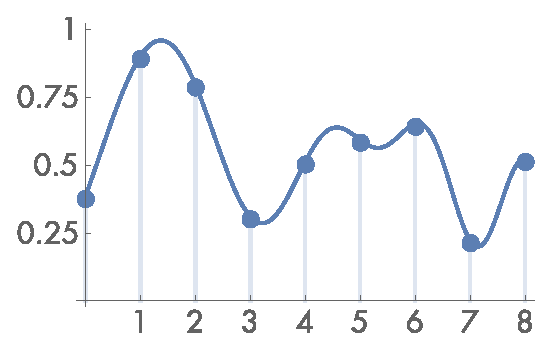
\includegraphics[width=0.4\linewidth]{chap07/point-sampling.eps}}\,\,
    \subfloat[]{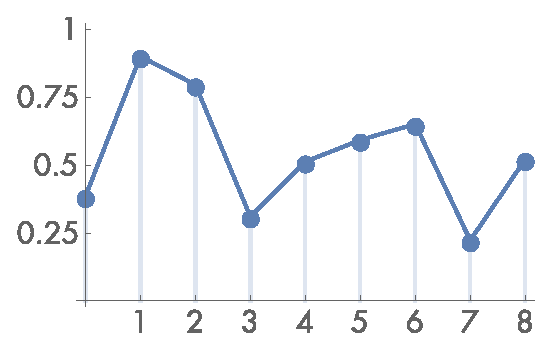
\includegraphics[width=0.4\linewidth]{chap07/linear-reconstruction.eps}}
    \caption{(a)通过取$f(x)$的\emph{样本点}集(标实心记),我们确定了函数在这些位置处的值。
        (b)样本值可用于\emph{重建}逼近$f(x)$的函数$\tilde{f}(x)$。
        \refsub{混叠}介绍的采样原理准确描述了关于$f(x)$的条件、
        所需样本的数目,以及使得$\tilde{f}(x)$和$f(x)$一模一样的重建技术。
        原始函数有时能只从样本点中完全重建的事实令人瞩目。}
    \label{fig:7.1}
\end{figure}

\keyindex{傅里叶分析}{Fourier analysis}{}可用于评估重建函数与原始函数间的匹配质量。
本节将用丰富细节来介绍一部分采样和重建过程中涉及的傅里叶分析主要思想,
但略去了许多性质的证明并跳过了与pbrt所用的采样算法没有直接关系的细节。
本章“扩展阅读”一节有关于这些话题详细信息的指引。

\subsection{频域与傅里叶变换}\label{sub:频域与傅里叶变换}
傅里叶分析的基础之一是\keyindex{傅里叶变换}{Fourier transform}{transform变换},
它在\keyindex{频域}{frequency domain}{}中来表示函数(我们称
通常的函数是在\keyindex{空域}{spatial domain}{}中表示的)。
考虑\reffig{7.2}中的两个函数。\reffig{7.2.1}中$x$的函数变化得相对较慢,
而\reffig{7.2.2}中的函数变化得迅速得多。称变化越慢的函数有越低频的分量。
\begin{figure}[htbp]
    \centering
    \subfloat[]{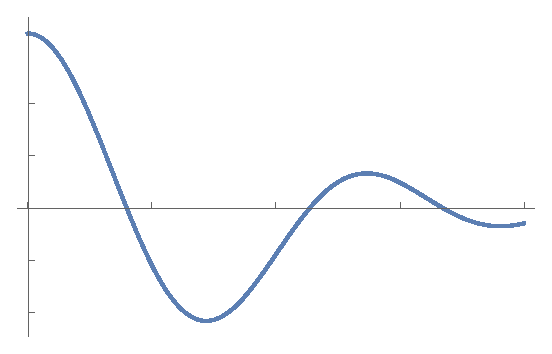
\includegraphics[width=0.32\linewidth]{chap07/func-lowfreq.eps}\label{fig:7.2.1}}\,\,\,\,
    \subfloat[]{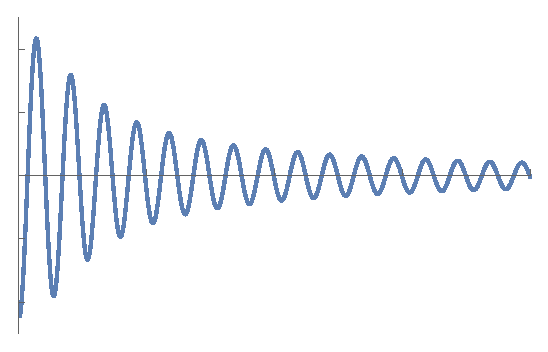
\includegraphics[width=0.32\linewidth]{chap07/func-highfreq.eps}\label{fig:7.2.2}}
    \caption{(a)低频函数和(b)高频函数。粗略地说,函数频率越高,在给定区域内变化得越快。}
    \label{fig:7.2}
\end{figure}

\reffig{7.3}展示了这两个函数在频率空间的表示;低频函数的表示比高频函数更快变为0。
\begin{figure}[htbp]
    \centering
    \subfloat[]{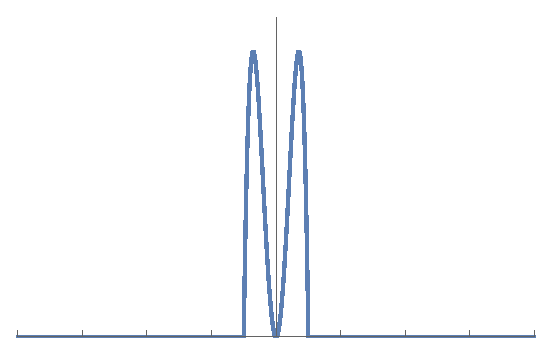
\includegraphics[width=0.32\linewidth]{chap07/fourier-lowfreq.eps}}\,\,\,\,
    \subfloat[]{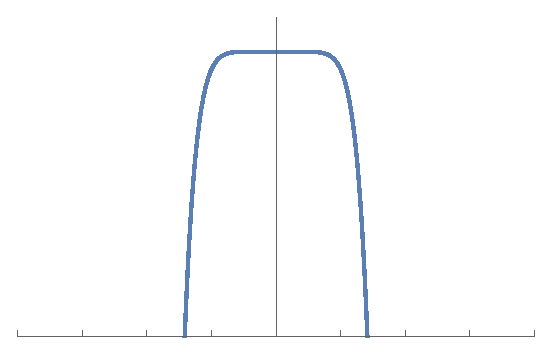
\includegraphics[width=0.32\linewidth]{chap07/fourier-highfreq.eps}}
    \caption{\reffig{7.2}中的函数的频率空间表示。本图展示了每个频率$\omega$对空域中每个函数的贡献。}
    \label{fig:7.3}
\end{figure}

许多函数可以分解为平移过的正弦曲线的加权和。
约瑟夫·傅里叶\sidenote{译者注:Jean-Baptiste Joseph Fourier,
    18至19世纪法国著名数学家和物理学家。其中文译名还常作“傅立叶”。}
首先描述了这一奇特事实,傅里叶变换即将函数转换为该表示。
函数的频率空间表示便于深入了解其一些特点——正弦函数的频率分布对应于原函数的频率分布。
使用该形式后,就能用傅里叶分析深入了解采样和重建过程引入的误差以及如何降低该误差带来的感知影响。

1D函数$f(x)$的傅里叶变换为\footnote{要告知读者的是,
    在不同领域中该积分前的常数并不总是一样的。例如一些作者(包括许多物理界的)
    更喜欢在两个积分前乘上$\frac{1}{\sqrt{2\pi}}$。}
\begin{align}\label{eq:7.1}
    F(\omega)=\int_{-\infty}^{\infty}f(x)\mathrm{e}^{-\mathrm{i}2\pi\omega x}\mathrm{d}x\, .
\end{align}
(回想$\mathrm{e}^{-\mathrm{i}x}=\cos x+\mathrm{i}\sin x$,其中$\mathrm{i}=\sqrt{-1}$。)
为了简便,这里我们将只考虑\keyindex{偶函数}{even function}{},
即$f(-x)=f(x)$,这种情况下$f$的傅里叶变换没有虚数项。
新函数$F$是\keyindex{频率}{frequency}{}$\omega$的函数
\footnote{本章中,我们将用符号$\omega$表示频率。在本书剩下部分中,$\omega$表示规范化的方向向量。
    这种记号的重复在使用它们的给定上下文中不应混淆。简单来说,当我们说函数的“频谱”(spectrum)时,
    我们是在说它在其频率空间表示中的频率分布,而不是和颜色相关的东西。}。
我们将用$\mathcal{F}$表示傅里叶变换运算
\sidenote{译者注:原文使用的符号是$\mathrm{F}$,这里译者换用更常用的花体$\mathcal{F}$,
    也更利于阅读时与其他符号区分。},即$\mathcal{F}\{f(x)\}=F(\omega)$。
$\mathcal{F}$显然是线性运算——即对任意标量$a$都有$\mathcal{F}\{af(x)\}=a\mathcal{F}\{f(x)\}$,
且$\mathcal{F}\{f(x)+g(x)\}=\mathcal{F}\{f(x)\}+\mathcal{F}\{g(x)\}$。

\refeq{7.1}称为\keyindex{傅里叶分析}{Fourier analysis}{}方程,有时简称\keyindex{傅里叶变换}{Fourier transform}{transform变换}。
我们也可用\keyindex{傅里叶合成}{Fourier synthesis}{}方程从频域变换回空域,
也称作\keyindex{傅里叶逆变换}{inverse Fourier transform}{transform变换}
\sidenote{译者注:大多数文献采用的傅里叶变换或逆变换定义中$\omega$是角频率,
    但本书的定义中$\omega$是频率。数值上角频率等于频率乘以$2\pi$。}:
\begin{align}\label{eq:7.2}
    f(x)=\int_{-\infty}^{\infty}F(\omega)\mathrm{e}^{\mathrm{i}2\pi\omega x}\mathrm{d}\omega\, .
\end{align}

\reftab{7.1}展示了许多重要函数及其频率空间表示
\sidenote{译者注:表中原文将频域函数写作$f(\omega)$,译者改为了$F(\omega)$。
    此外,表中原文对余弦函数和shah函数的频域表示混用了系数不同的傅里叶变换定义,
    导致与本书所采用的定义不符,译者已根据本书定义对其作了修正。
    具体推导过程可参考译者补充的\refsec{译者补充:信号处理}。}。
这些函数中许多都基于狄拉克$\delta$分布
\sidenote{译者注:也称作单位\keyindex{冲激函数}{impulse function}{}、脉冲函数。},
该空间函数的定义使得$\displaystyle\int_{-\infty}^{\infty}\delta(x)\mathrm{d}x=1$,且对任意$x\neq0$,都有$\delta(x)=0$。
这些性质的一个重要结论是\sidenote{译者注:我在原文基础上为该式加上了积分上下限以表明它是定积分。}
\begin{align*}
    \int_{-\infty}^{\infty} f(x)\delta(x)\mathrm{d}x=f(0)\, .
\end{align*}

$\delta$分布不能表示为标准数学函数,但通常可以视作以原点为中心且宽度逼近0的
单位面积矩形函数\sidenote{译者注:原文box function。}的极限。
\begin{table}[htbp]
    \centering\begin{tabular}{l p{170pt}}
        \toprule
        {\bfseries 空域}                                                   & {\bfseries 频率空间表示}                                                                     \\
        \midrule
        矩形函数:$f(x)=\left\{\begin{array}{ll}
                1, & \text{若}|x|<\frac{1}{2}, \\
                0, & \text{其他}.
            \end{array}\right.$           & sinc函数:$\displaystyle F(\omega)=\mathrm{sinc}(\omega)=\frac{\sin(\pi\omega)}{\pi\omega}$  \\
        \hline
        高斯函数:$f(x)=\mathrm{e}^{-\pi x^2}$                             & 高斯函数:$F(\omega)=\mathrm{e}^{-\pi \omega^2}$                                             \\
        \hline
        常函数:$f(x)=1$                                                   & $\delta$函数:$F(\omega)=\delta(\omega)$                                                     \\
        \hline
        余弦函数:$f(x)=\cos x$                                            & 平移的$\delta$函数:
        $F(\omega)=\frac{1}{2}(\delta(1-2\pi\omega)+\delta(1+2\pi\omega))$                                                                                                \\
        \hline
        shah函数:$\displaystyle f(x)=III_T(x)=T\sum\limits_k\delta(x-kT)$ & $\displaystyle F(\omega)=TIII_{\frac{1}{T}}(\omega)=\sum\limits_k\delta(\omega-\frac{k}{T})$ \\
        \bottomrule
    \end{tabular}
    \caption{傅里叶变换对。空域中的函数及其频率空间表示。
        因为傅里叶变换的对称性,如果左边一列被当作频率空间,
        则右边一列是这些函数的空间等价。}
    \label{tab:7.1}
\end{table}

\subsection{理想采样与重建}\label{sub:理想采样与重建}
利用频率空间分析,我们现在能正式研究采样的性质了。
回想采样过程要求我们选择一组等间隔样本位置并计算这些位置的函数值。
形式上,这对应于让该函数乘以“shah”——或称“冲激串”函数
\sidenote{译者注:也称狄拉克梳状函数。},即无数等间隔的$\delta$函数之和。
shah函数$III_T(x)$定义为\sidenote{译者注:为了和虚数单位$\mathrm{i}$更好区分,
    译者将式子中的下标$i$改为$k$,下同。}
\begin{align*}
    III_T(x)=T\sum\limits_{k=-\infty}^{\infty}\delta(x-kT)\, ,
\end{align*}
其中$T$定义了\keyindex{周期}{period}{},也称\keyindex{采样率}{sampling rate}{}。
\reffig{7.4}展示了采样的正式定义。相乘后得到函数在等间隔点处取值的无限序列:
\begin{align*}
    III_T(x)f(x)=T\sum\limits_k\delta(x-kT)f(kT)\, .
\end{align*}
\begin{figure}[htbp]
    \centering
    \subfloat[]{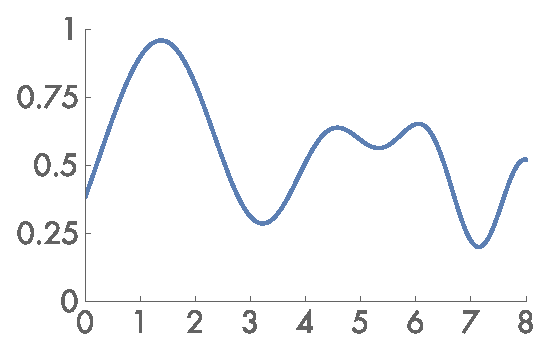
\includegraphics[width=0.32\linewidth]{chap07/func-to-sample.eps}}\,
    \subfloat[]{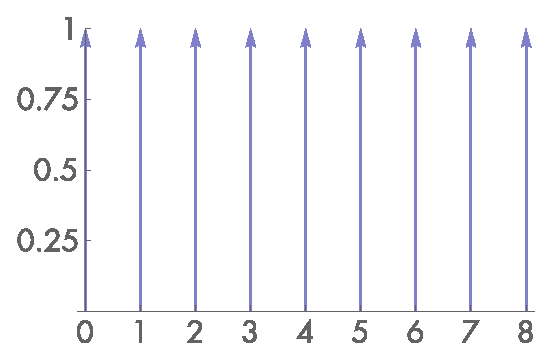
\includegraphics[width=0.32\linewidth]{chap07/shah-samples.eps}}\,
    \subfloat[]{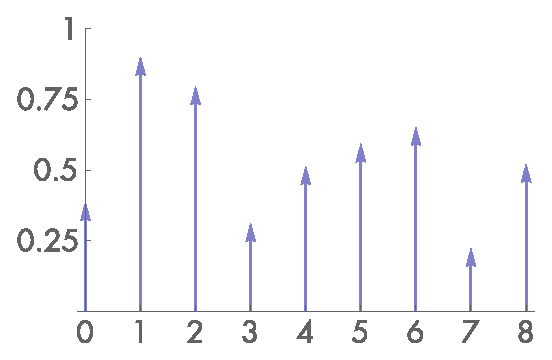
\includegraphics[width=0.32\linewidth]{chap07/shah-sampled-function.eps}}
    \caption{形式化的采样过程。(a)函数$f(x)$乘以(b)shah函数$III_T(x)$,
        得到(c)表示其在每个样本点处取值的缩放后的$\delta$函数的无限序列。}
    \label{fig:7.4}
\end{figure}

通过选择重建滤波器函数$r(x)$并计算\keyindex{卷积}{convolution}{},
这些样本值可用于定义重建的函数$\tilde{f}$,即
\begin{align*}
    (III_T(x)f(x))\otimes r(x)\, ,
\end{align*}
其中卷积运算$\otimes$定义为
\begin{align*}
    f(x)\otimes g(x)=\int_{-\infty}^{\infty}f(x')g(x-x')\mathrm{d}x'\, .
\end{align*}

对于重建,卷积给出以样本点为中心并缩放后的重建滤波器实例加权和:
\begin{align*}
    \tilde{f}(x)=T\sum\limits_{k=-\infty}^{\infty}f(kT)r(x-kT)\, .
\end{align*}

例如\reffig{7.1}中使用了三角形重建滤波器$r(x)=\max(0,1-|x|)$。
\reffig{7.5}展示了为该例所用的缩放后的三角形函数。
\begin{figure}[htbp]
    \centering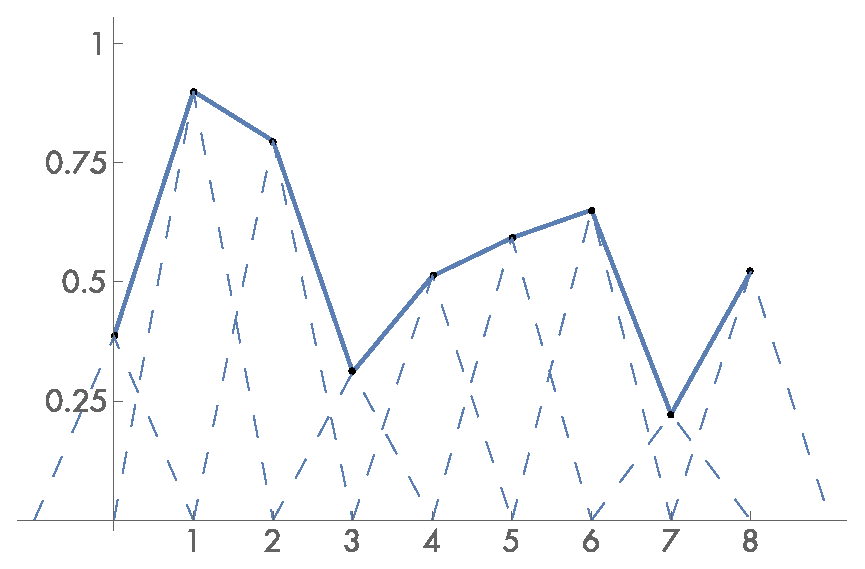
\includegraphics[width=0.6\linewidth]{chap07/func-tri-reconstruction.eps}
    \caption{虚线表示的三角形重建滤波器实例的和给出了实线表示的对原始函数的重建逼近。}
    \label{fig:7.5}
\end{figure}

为了得到直观的结果,我们经历了看似不用这么复杂的过程:
用一些方法在样本间插值也能得到重建函数$\tilde{f}(x)$。
然而通过仔细构建这些背景,傅里叶分析现在能更简单地用于该过程。

通过在频域分析采样函数,我们能更深入理解采样过程。
特别地,我们将能确定原始函数能从其在样本位置的取值中完全恢复的条件——一个很强的结论。
对于此处的讨论,我们现在假设函数$f(x)$是\keyindex{带限}{band limited}{}的——
存在某个频率$\omega_0$使得$f(x)$在大于$\omega_0$处不再包含任何频率。
根据定义,带限函数具有紧支撑\sidenote{译者注:compact support。}的频率空间表示,
即对于所有$|\omega|>\omega_0$都有$F(\omega)=0$。\reffig{7.3}中的两个频谱都是带限的。

傅里叶分析所用的一个重要思想是两个函数之积的傅里叶变换$\mathcal{F}\{f(x)g(x)\}$可
表示为它们各自傅里叶变换$F(\omega)$和$G(\omega)$的卷积:
\begin{align*}
    \mathcal{F}\{f(x)g(x)\}=F(\omega)\otimes G(\omega)\, .
\end{align*}

类似地,空域卷积等价于频域乘积:
\begin{align}\label{eq:7.3}
    \mathcal{F}\{f(x)\otimes g(x)\}=F(\omega)G(\omega)\, .
\end{align}

这些性质是傅里叶分析的标准参考文献中得来的。
利用这些思想可以发现,空域中原始的采样步骤,即shah函数与原始函数$f(x)$相乘,
可等价描述为频域中$F(\omega)$与另一shah函数的卷积。

从\reftab{7.1}中我们还知道shah函数$III_T(x)$的频谱;
周期为$T$的shah函数的傅里叶变换是另一个周期为$\displaystyle\frac{1}{T}$的shah函数。
牢记周期间的倒数关系很重要:它意味着如果样本在空域中隔得较远,
则它们在频域中离得更近。

因此采样信号的频域表示通过$F(\omega)$和新的shah函数的卷积给出。
让$\delta$函数与一个函数卷积得到该函数副本,故用shah函数卷积
得到原始函数副本的无限序列,间隔等于该shah的周期(\reffig{7.6})。
它是样本序列的频率空间表示。
\begin{figure}[htbp]
    \centering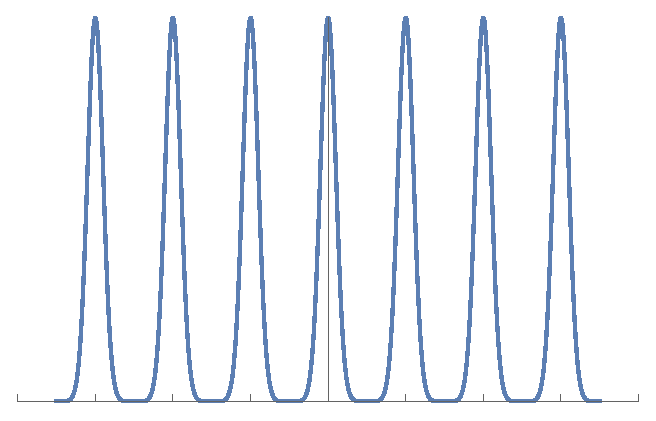
\includegraphics[width=0.45\linewidth]{chap07/func-convolve-shah.eps}
    \caption{$F(\omega)$与shah函数的卷积。结果是$F$的无数个副本。}
    \label{fig:7.6}
\end{figure}

现在我们有了该函数频谱副本的无限集,我们该怎样重建原始函数呢?
观察\reffig{7.6},答案很明显:只需要抹除除了以原点为中心外的所有频谱副本,就能得到原始的$F(\omega)$.
\begin{figure}[htbp]
    \centering
    \subfloat[]{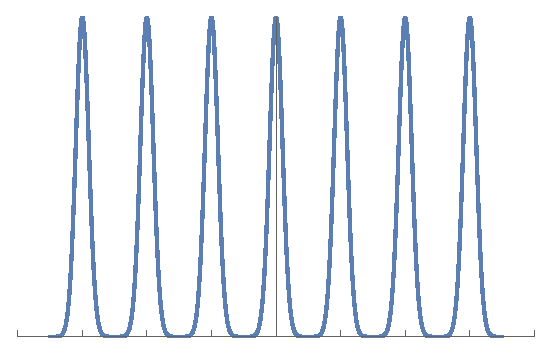
\includegraphics[width=0.32\linewidth]{chap07/func-convolve-shah-a.eps}}\,
    \subfloat[]{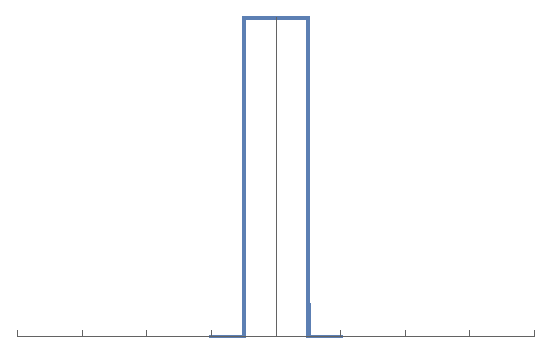
\includegraphics[width=0.32\linewidth]{chap07/unit-box-filter.eps}}\,
    \subfloat[]{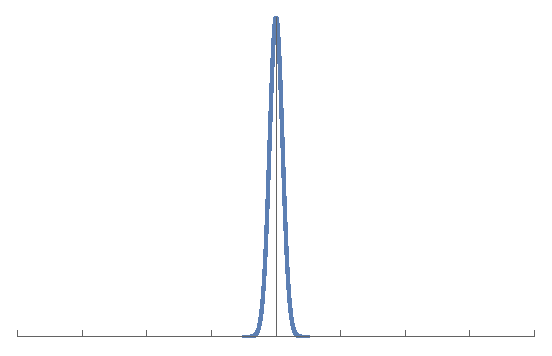
\includegraphics[width=0.32\linewidth]{chap07/single-func-after-box.eps}}
    \caption{(a)$F(\omega)$的副本序列和(b)合适的矩形函数相乘得到(c)原始频谱。}
    \label{fig:7.7}
\end{figure}

为了丢弃除了中间外的所有频谱副本,我们乘以具有合适宽度的矩形函数(\reffig{7.7})。
宽度为$T$的矩形函数$\textstyle\prod_T(x)$定义为
\begin{align*}
    {\textstyle\prod_T}(x)=\left\{\begin{array}{ll}
        \displaystyle\frac{1}{T}, & \text{若}\displaystyle|x|<\frac{T}{2}, \\
        0,                        & \text{其他}.
    \end{array}\right.
\end{align*}

该相乘步骤对应了用重建滤波器在空域做卷积。这是理想采样与重建过程。总结为:
\begin{align*}
    \tilde{F}=(F(\omega)\otimes III_{\frac{1}{T}}(\omega))\textstyle\prod_{\frac{1}{T}}(\omega)\, .
\end{align*}

这是个重要结论:仅仅通过采样一组均匀间隔的点,我们就能确定$f(x)$的精准频率空间表示。
除了知道该函数是带限的外,没有使用关于函数成分的额外信息。

在空域运用等价过程同样能完全恢复$f(x)$。因为矩形函数的傅里叶逆变换是sinc函数,
所以空域中的理想重建是\sidenote{译者注:原文该式继承了\reftab{7.1}的错误,
这里笔者补回了第一项的系数$\frac{1}{T}$。}
\begin{align*}
    \tilde{f}=\left(\frac{1}{T}f(x)III_T(x)\right)\otimes \mathrm{sinc}_T(x)\, ,
\end{align*}
其中$\mathrm{sinc}_T(x)=\mathrm{sinc}(Tx)$,因此\sidenote{译者注:原文该式
将$\mathrm{sinc}_T(x-kT)$误写为$\mathrm{sinc}(x-kT)$,已修正。}
\begin{align*}
    \tilde{f}(x)=\sum\limits_{k=-\infty}^{\infty}\mathrm{sinc}_T(x-kT)f(kT)\, .
\end{align*}

不幸的是,因为sinc函数有无限定义域,所以必须用所有采样值$f(kT)$来计算空域中$\tilde{f}(x)$的任一特定值。
实际实现中更爱用空间范围有限的滤波器,即使它们不能完美重建原始函数。

图形学常用的可选方法是用矩形函数做重建,即高效地对$x$附近区域内的全部样本值做平均。
通过考虑矩形滤波器的频域表现可以看到这是非常糟糕的选择:
该技术试图通过\emph{乘以sinc}来分离出函数频谱中间的副本,
这不仅在选出函数频谱中央副本方面做得很差,
还包含了无限序列中其他副本的高频贡献。

\subsection{混叠}\label{sub:混叠}
除了sinc函数无限定义域的问题外,理想采样与重建方法一个最严重的实际问题是它假设信号是带限的。
对于非带限信号,或者没能以足够高的采样率采样其频率成分的信号,
之前描述的过程会重建出与原始信号不同的函数。

成功重建的关键是用宽度合适的矩形函数相乘以完全恢复原始频谱$F(\omega)$的能力。
注意在\reffig{7.6}中,信号频谱的副本被空白空间分隔,所以能够被完美重建。
然而如果以更低的采样率采样原始函数,考虑一下会发生什么。
回想周期为$T$的shah函数$III_T$的傅里叶变换是周期为$\displaystyle\frac{1}{T}$的新shah函数。
这意味着如果空域中样本间的距离增大,频域的样本间隔会变小,
将频谱$F(\omega)$的副本挤在一起。如果副本挨得太近,它们就开始重叠。

因为副本被加在一起,所以得到的频谱看起来不再像许多原始的副本(\reffig{7.8})。
当该新频谱乘以矩形函数后,结果是相似但不等于原始$F(\omega)$的频谱:
原始信号的高频细节渗入到重建信号频谱的低频区域。
这些新的低频伪影称作\keyindex{混叠}{alias}{}(因为高频“伪装”成低频),
得到的信号被称是\keyindex{混叠的}{aliased}{alias混叠}。
\begin{figure}
    \centering
    \subfloat[]{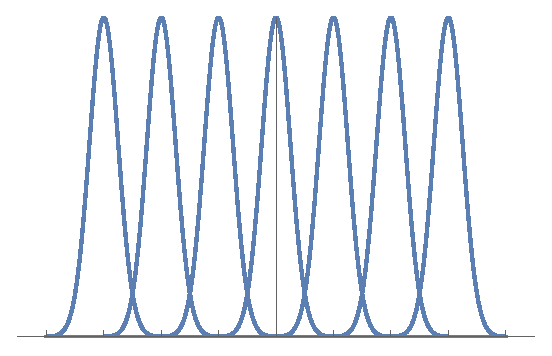
\includegraphics[width=0.4\linewidth]{chap07/freq-space-overlap.eps}}\,
    \subfloat[]{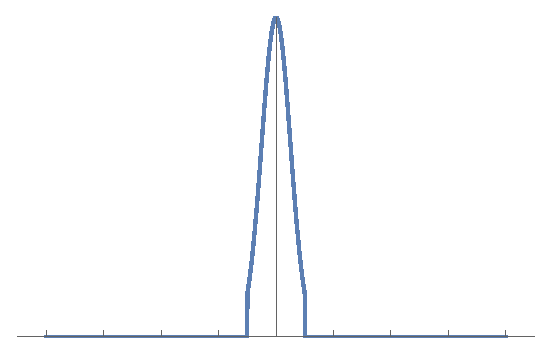
\includegraphics[width=0.4\linewidth]{chap07/freq-space-aliasing.eps}}
    \caption{(a)采样率过低时,函数频谱副本会重叠,当执行重建时会导致(b)混叠。}
    \label{fig:7.8}
\end{figure}

\reffig{7.9}\sidenote{译者注:原文该图题注函数表达式有笔误,已修正。}
展示了欠采样并重建1D函数$f(x)=1+\cos(4\pi x^2)$时的混叠效应。
\begin{figure}[htbp]
    \centering
    \subfloat[]{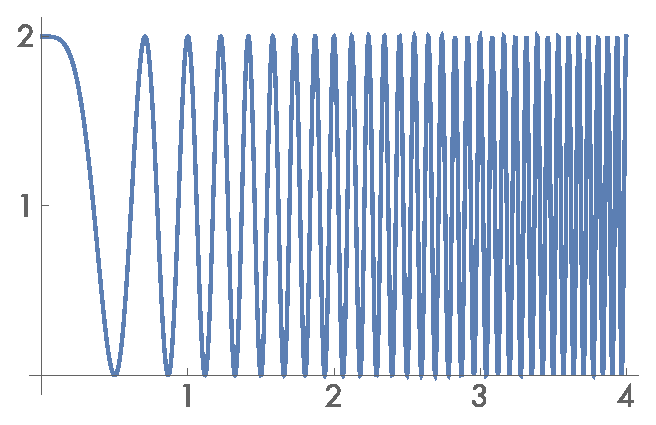
\includegraphics[width=0.4\linewidth]{chap07/freq-increasing-func.eps}}\,
    \subfloat[]{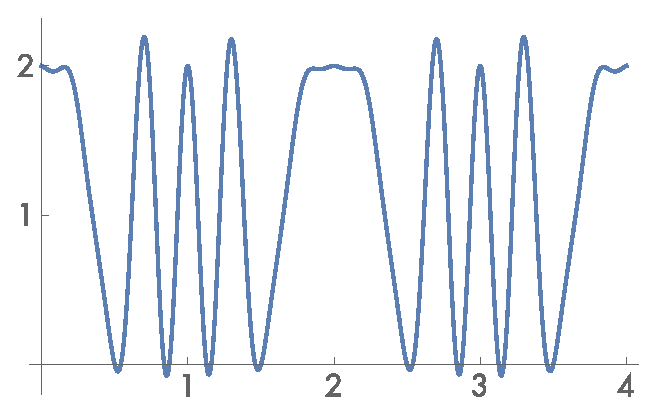
\includegraphics[width=0.4\linewidth]{chap07/freq-increasing-aliased.eps}}
    \caption{函数$f(x)=1+\cos(4\pi x^2)$采样点的混叠。(a)该函数。
        (b)以0.125单位为样本间隔采样并用sinc滤波器执行完美重建后所重建出的函数。
        混叠造成原始函数的高频信息被丢失了并作为低频误差重新出现。}
    \label{fig:7.9}
\end{figure}

一种可能解决重叠频谱问题的办法是简单地增加采样率
直到频谱的副本隔得足够远而不再重叠,进而完全消除混叠。
事实上,\keyindex{采样定理}{sampling theorem}{}准确告诉我们所需的采样率。
该定理说只要均匀样本点的频率$\omega_s$大于信号中出现的最大频率$\omega_0$的两倍,
就能从样本中完美重建原始信号。该最小采样频率称为\keyindex{奈奎斯特频率}{Nyquist frequency}{frequency频率}
\sidenote{译者注:哈里·奈奎斯特(Harry Nyquist),19至20世纪瑞典裔美国著名物理学家,通讯理论的奠基者之一。}。

对于非带限信号($\omega_0=\infty$),不可能以足够高的采样率执行完美重建。
非带限信号有无限支撑的频谱,所以无论其频谱副本隔得多远(即无论我们用多高的采样率),
都总会有重叠。不幸的是,计算机图形学中要处理的函数很少是带限的。
特别地,任何不连续的函数都不是带限的,因此我们不能完美采样和重建它。
这是有道理的,因为两个样本间的函数连续性是不清楚的,样本没有提供不连续处的信息。
因此除了提高采样率外还必须用不同方法来消除混叠可能引入到渲染器结果中的误差。

\subsection{抗锯齿技术}\label{sub:抗锯齿技术}
如果不仔细对待采样和重建,则最终图像中可能出现大量伪影。
有时区分采样伪影与重建伪影很有用;确切地说,我们会称采样伪影为\keyindex{预混叠}{prealiasing}{alias混叠},
称重建伪影为\keyindex{后混叠}{postaliasing}{alias混叠}。任意想要修正这些误差的尝试都
大体划分为\keyindex{抗锯齿}{antialiasing}{}\sidenote{译者注:也称反混叠。}。
本节将回顾除了只增加采样率外的大量抗锯齿技术。

\subsubsection*{非均匀采样}
尽管知道我们要采样的图像函数有无穷的频率成分因而不能从样本点中完美重建,
但以非均匀的方式改变样本间隔有可能降低混叠的视觉影响。
如果$\xi$表示在0到1间的随机数,则基于冲激串的非均匀样本集为
\begin{align*}
    \sum\limits_{k=-\infty}^{\infty}\delta\left(x-(k+\frac{1}{2}-\xi)T\right)\, .
\end{align*}

对于不足以刻画该函数的固定采样率,均匀和非均匀采样都会得到不正确的重建信号。
然而非均匀采样倾向于将规则的混叠伪影转化为不容易引起人类视觉系统注意的噪声。
在频率空间,采样信号的副本最终也被随机平移,
所以当执行重建时结果是随机误差而不是有条理的混叠。

\subsubsection*{自适应采样}
另一个对抗混叠的建议方法是\keyindex{自适应超采样}{adaptive supersampling}{}:
如果我们能辨别出频率高于奈奎斯特上限的信号区域,
则我们可以在这些区域再取额外样本而不用承担在每处都增加采样频率所致的计算开销。
在实际中让该方法奏效是很困难的,因为寻找所有需要超采样的地方会很难。
大多数这样做的技术都基于测试相邻样本值并找到两值间有明显变化的地方;
然后假设该区域信号有较高频率。

通常相邻样本值不能确定地告诉我们它们之间到底发生了什么:
即使它们值相同,函数也可能在它们间有巨大变化。
或者相邻样本可能有相差很大的值但实际上并没有出现任何混叠。
例如,第\refchap{纹理}的纹理滤波算法全力消除场景中图像贴图和表面过程纹理造成的混叠;
我们不想让自适应采样例程在纹理值迅速变化但实际上没有出现过高频率的区域不必要地采额外样本。

\subsubsection*{预滤波}
采样理论提供的另一个消除混叠的方法是对原始函数滤波(即模糊)
使得所用采样率不能精确捕获的高频率不再保留下来。
该方法应用于第\refchap{纹理}的纹理函数。
该技术通过从被采样函数中移除信息来改变其特性,模糊一般不如混叠令人讨厌。

回想我们要用选定宽度的矩形滤波器与原始函数频谱相乘使得
奈奎斯特上限之上的频率被移除。在空域,这对应于原始函数与sinc滤波器做卷积,
\begin{align*}
    f(x)\otimes \mathrm{sinc}(2\omega_sx)\, .
\end{align*}

在实际中,我们也可以用范围有限的滤波器。该滤波器的频率空间表示能
帮助弄清它能有多逼近理想sinc滤波器的表现。

\reffig{7.10}展示了函数$1+\cos(4\pi x^2)$与\refsec{图像重建}
介绍的范围有限的sinc变种的卷积\sidenote{译者注:原文正文与插图
    题注的函数表达式均有笔误,与图示不符,译者已修改。}。
注意高频细节被消除了;该函数可用\reffig{7.9}的采样率采样和重建而无混叠。
\begin{figure}[htbp]
    \centering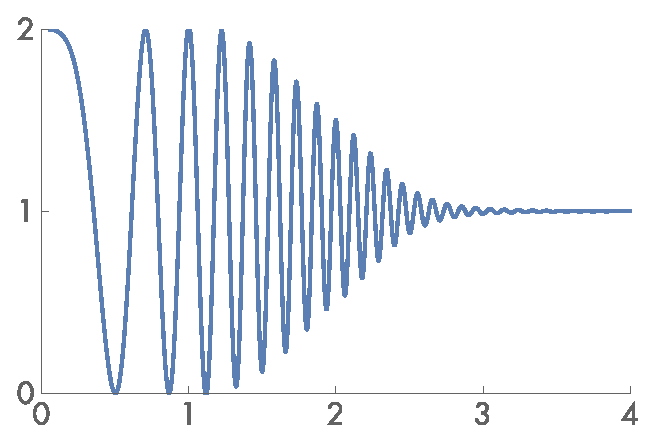
\includegraphics[width=0.4\linewidth]{chap07/highfreq-prefiltered.eps}
    \caption{函数$1+\cos(4\pi x^2)$与移除采样率$T=0.125$对应的
        奈奎斯特上限之外频率的滤波器的卷积。高频细节已从该函数移除掉,
        使得新函数至少能无混叠地被采样与重建。}
    \label{fig:7.10}
\end{figure}

\subsection{应用到图像合成}\label{sub:应用到图像合成}
这些思想应用到2D情况的渲染场景的图像采样和重建很简单:
我们有一张图像可视作2D图像位置$(x,y)$到辐亮度值$L$的函数:
\begin{align*}
    f(x,y)\rightarrow L\, .
\end{align*}

好消息是,有了我们的光线追踪器,我们能在我们所选的任意点$(x,y)$处求该函数的值。
坏消息是,一般不太可能在采样前对$f$预滤波来从中移除高频。
因此本章采样器使用两种策略,既将采样率提升至超过最终图像基础像素间隔,
也有非均匀分布样本以将混叠转化为噪声。

将场景函数的定义推广为也依赖于时间$t$以及采样处的透镜位置$(u,v)$的更高维函数很有用。
因为来自相机的光线基于这五个量,它们中任意一个变化都会得到不同的光线,
进而可能是不同的$f$值。对于特定的图像位置,该点的辐亮度一般
随时间(如果场景中有运动物体)和透镜上的位置(如果相机有光圈有限的透镜)变化。

更一般地,因为第\refchap{光传输I:表面反射}到第\refchap{光传输III:双向方法}
定义的许多积分器都用统计技术来估计沿给定光线的辐亮度,
所以当重复给定相同光线时它们可能返回不同的辐亮度值。
如果我们进一步将场景辐亮度函数扩展至包含积分器所用的样本值
(例如,为了照明计算而用于在面光源上选点的值),
我们就有甚至更高维的图像函数
\begin{align*}
    f(x,y,t,u,v,i_1,i_2,\ldots)\rightarrow L\, .
\end{align*}

采样好所有这些维度是高效生成高质量图像的重要一部分。
例如如果我们保证图像上位置$(x,y)$附近倾向于在透镜上有不同的$(u,v)$,
则得到的渲染图像会有更小的误差,因为每个样本更有可能考虑了其相邻样本没有考虑的场景信息。
后面几节的类\refvar{Sampler}{}会解决高效采样所有这些维度的问题。

\subsection{渲染中的混叠来源}\label{sub:渲染中的混叠来源}
几何体是在渲染图像中造成混叠的最常见因素之一。
当投影到图像平面时,物体的边界引入了\keyindex{阶跃函数}{step function}{}——
图像函数的值突然从一个值跳到另一个值。
不仅阶跃函数像前面所述那样有无穷的频率成分,
而且更糟糕的是,完美重建滤波器在运用于混叠样本时也会造成伪影:
重建函数中出现\keyindex{振铃}{ringing}{}伪影,
即称作\keyindex{吉布斯现象}{Gibbs phenomenon}{}的效应。
\reffig{7.11}为1D函数展示了该效应的例子。
正如我们将在本章后续所看到的,选择有效的重建滤波器来面对混叠需要科学、艺术以及个人品味。
\begin{figure}[htbp]
    \centering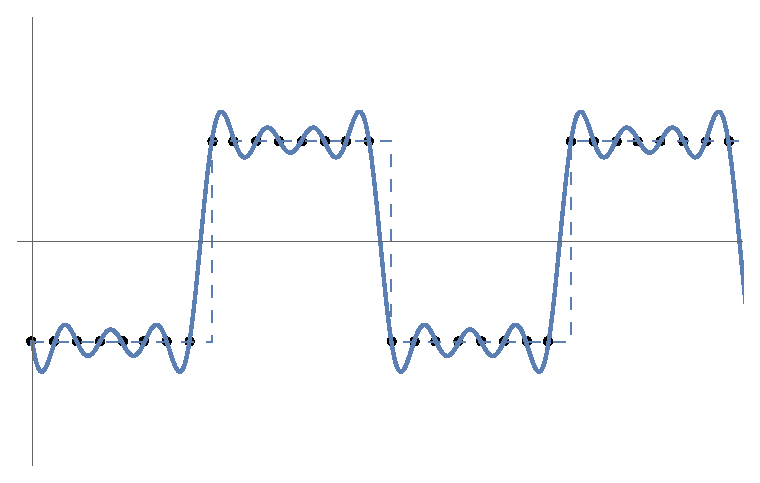
\includegraphics[width=0.5\linewidth]{chap07/gibbs-phenomenon.eps}
    \caption{吉布斯现象的图示。当没有以奈奎斯特采样率采样函数却又用
        sinc滤波器重建一组混叠的样本时,重建的函数会有“振铃”伪影,它在真实函数附近振荡。
        这里用0.125的样本间隔采样1D阶跃函数(虚线)。当用sinc重建时,振铃出现了(实线)。}
    \label{fig:7.11}
\end{figure}

场景中非常小的物体也会造成几何混叠。如果几何体小到落入图像平面样本之间,
则它会在一个动画的若干帧中不可预测地消失和重现。

混叠的另一个来源可能来自物体上的纹理和材质。没有被正确滤波的纹理贴图
(解决该问题是第\refchap{纹理}的主要内容)或光泽表面的小高光
可能造成\keyindex{着色混叠}{shading aliasing}{alias混叠}。
如果采样率没有高到足以充分采样这些特征,则会导致混叠。
此外,一个物体投射的尖锐阴影会在最终图像中引入另一个阶跃函数。
尽管有可能从图像平面上的几何边来辨别阶跃函数的位置,
但从阴影边界中检测阶跃函数则更加困难。

对于渲染图像中混叠的关键认识是,我们永远不可能移除所有这些来源,
所有我们必须开发技术来减轻其对最终图像质量的影响。

\subsection{理解像素}\label{sub:理解像素}
在本章剩余内容中牢记两个关于像素的观点很重要。
第一,一定记住构成图像的像素是图像函数在图像平面上离散位置的样本点;这样的像素没有相应的“面积”。
正如\citet{Smith95apixel}着重指出的,将像素视作具有有限面积的小方形是错误的认知模型,
会导致一系列问题。通过用信号处理的方法介绍本章话题,我们尝试为更准确的认知模型奠定基础。

第二个问题是最终图像中的像素是在像素网格上的离散整数坐标$(x,y)$处自然定义的,
但本章的\refvar{Sampler}{}是在连续的浮点位置$(x,y)$处生成图像样本的。
映射这两个域的自然方法是将连续坐标舍入到最近的离散坐标;
既然它把刚好和离散坐标有相同值的连续坐标就映射为那个离散坐标,该方法看起来不错。
然而结果是,给定覆盖范围$[x_0,x_1]$的离散坐标集,则连续坐标集覆盖范围为$\displaystyle[x_0-\frac{1}{2},x_1+\frac{1}{2})$。
因此任何为给定离散像素范围生成连续样本位置的代码都被$\displaystyle\frac{1}{2}$的偏移量扰乱。
它们很容易被忘记并导致隐晦的错误。

如果我们改用
\begin{align*}
    d=\lfloor c\rfloor\, ,
\end{align*}
将连续坐标$c$截断为离散坐标$d$,并通过
\begin{align*}
    c=d+\frac{1}{2}\, ,
\end{align*}
将离散转换为连续,则离散范围$[x_0,x_1]$对应的连续坐标范围
自然是$[x_0,x_1+1)$且所得代码会简单得多\citep{HECKBERT1990246}。
\reffig{7.12}展示了我们将在pbrt中采用的这一转化。
\begin{figure}[htbp]
    \centering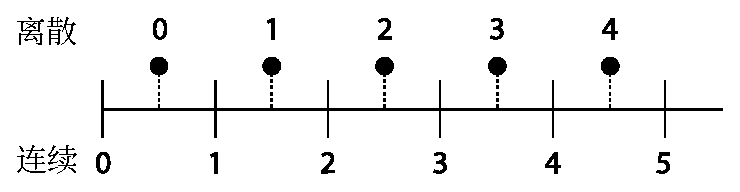
\includegraphics[width=0.5\linewidth]{chap07/Pixelsdiscretecontinuous.eps}
    \caption{图像中的像素可以解释为\emph{离散}或\emph{连续}坐标。
    离散图像五个像素的宽度覆盖了连续像素范围$[0,5)$。
    特定离散像素$d$的坐标在连续表示中为$\displaystyle d+\frac{1}{2}$。}
    \label{fig:7.12}
\end{figure}